\documentclass{beamer}
\usepackage{graphicx}
%%
\title{Uncertainties in precipitation
estimates from space-borne radar observations}
\author{Mircea Grecu}
\institute{NASA Goddard Space Flight Center and Morgan State University}
\date{March 2,2023}
%%\date{\today}

\begin{document}
\frame{\titlepage}
\begin{frame}
\frametitle{Sources of uncertainties}
\begin{columns}
%%in the precipitation estimates from space-borne radar observations
\begin{column}{0.45\textwidth}
    Major sources of uncertainty include:
    \begin{itemize}
        \item Variability in the Z-R relationships
        \item Attenuation in the observed radar reflectivity
        \item Variability in the radar beam footprint
        \item Ground clutter
    \end{itemize}
\end{column}
\begin{column}{0.55\textwidth}  %%<--- here
    \begin{figure}
    \begin{center}
     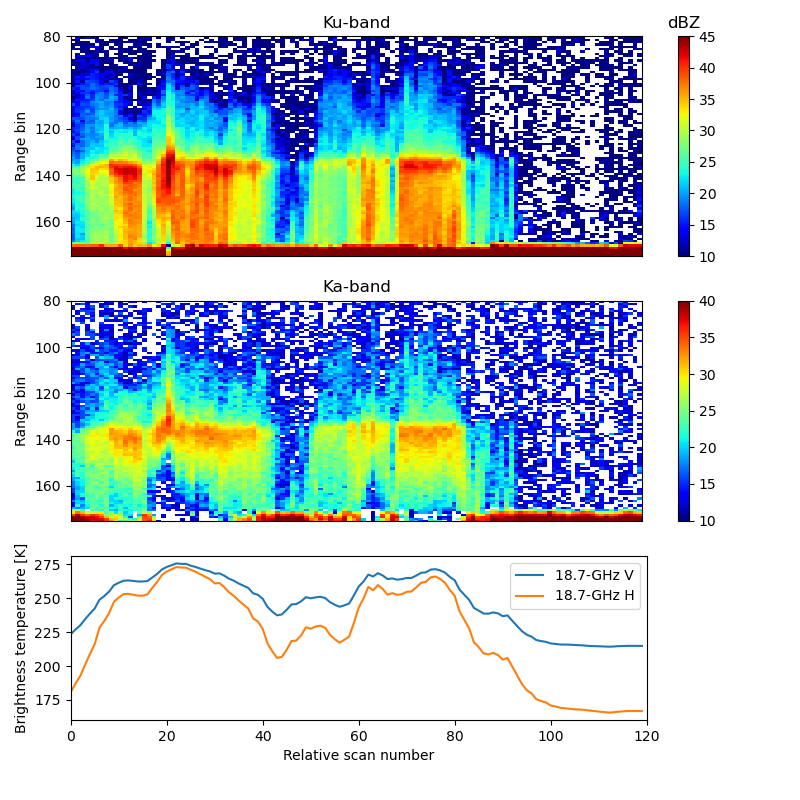
\includegraphics[width=0.9\textwidth]{Figures/fig1.png}
     \end{center}
    \end{figure}
\end{column}
\end{columns}
\end{frame}
\begin{frame}
\frametitle{Variability in the Z-Precipitation Rate relationships}
\begin{itemize}
    \item At least 2 parameters are required to describe
    Particle size distributions (PSDs).
    \item Consequently, the Z-Precipitation Rate relationships require at
    least 2 parameters. The generalized PSD intercept, $N_w=\frac {4^4} {\pi \rho_w} \frac {PWC} {D_m^4}$,
    greatly simplify Z-Rate relationships.
\end{itemize}
\begin{figure}
\begin{center}
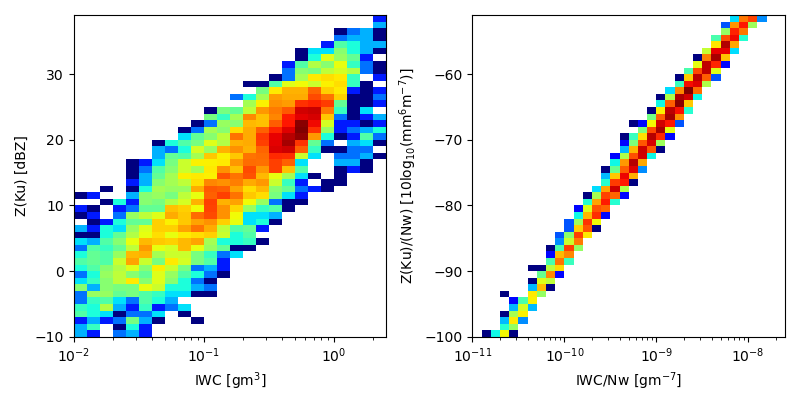
\includegraphics[width=0.9\textwidth]{Figures/fig2.png}
\end{center}
\end{figure}
\end{frame}
\begin{frame}
\frametitle{The $N_w$ problem. General considerations}
\begin{columns}
    \begin{column}{0.5\textwidth}
        \begin{itemize}
            \item The $N_w$ parameter greatly simplifies the formulation, but
            not the problem.
            \item It does not solve it though, as $N_w$ still needs to
            estimated independently of the radar observations.
            \item Ground observations may be used to impose constraints on
            $N_w$.
            \item However, such constraints are not very effective for 
            PSD characterized by large mean particle sizes $D_m$.
        \end{itemize}
    \end{column}
    \begin{column}{0.5\textwidth}
        \begin{figure}
            \begin{center}
            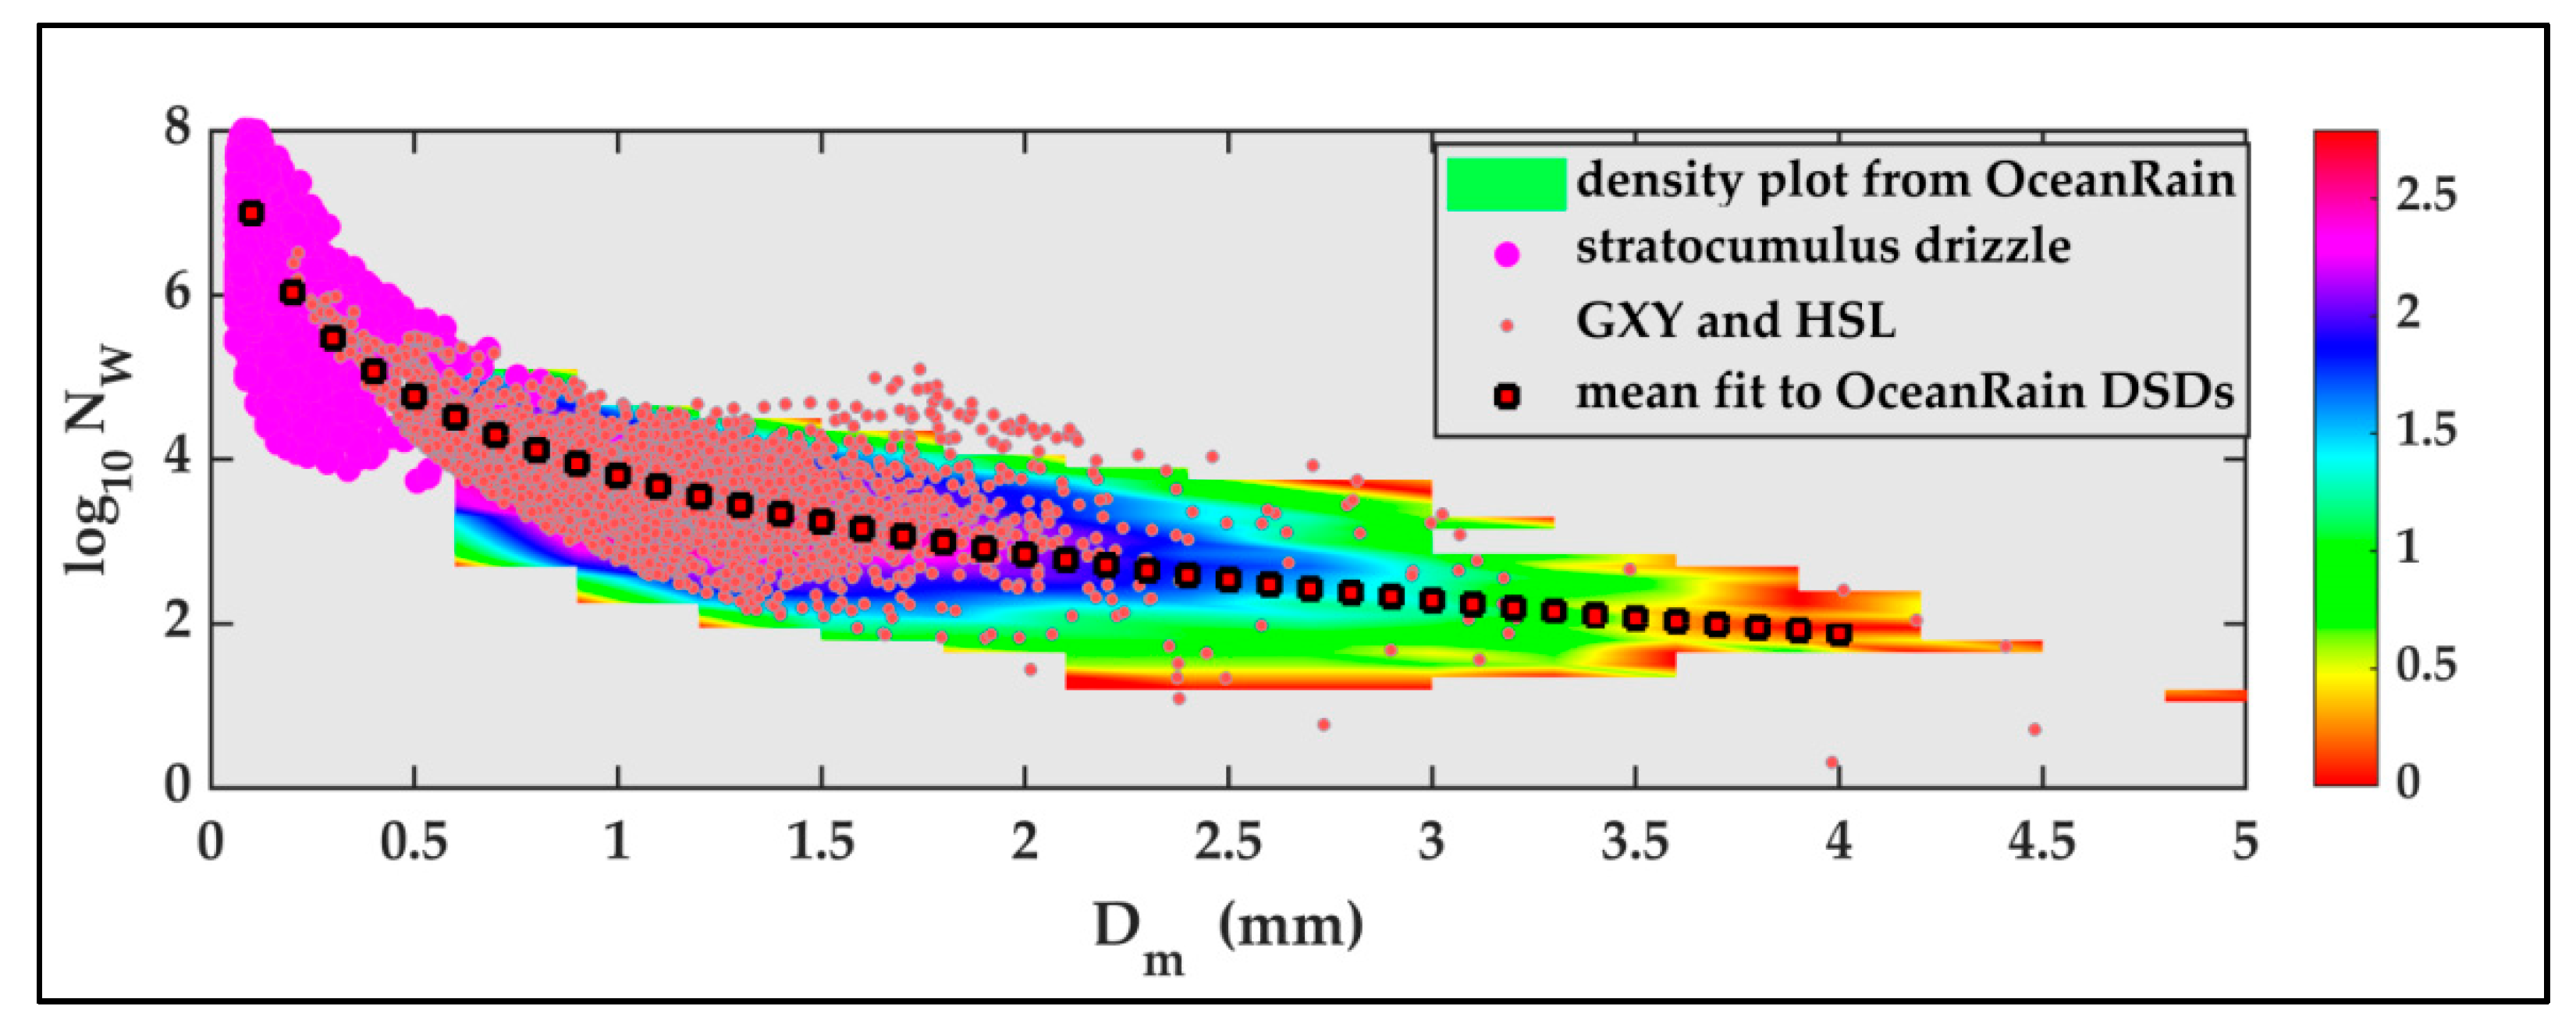
\includegraphics[width=0.9\textwidth]{Figures/fig3.png}
            \end{center}
        \end{figure}
        \begin{figure}
            \begin{center}
            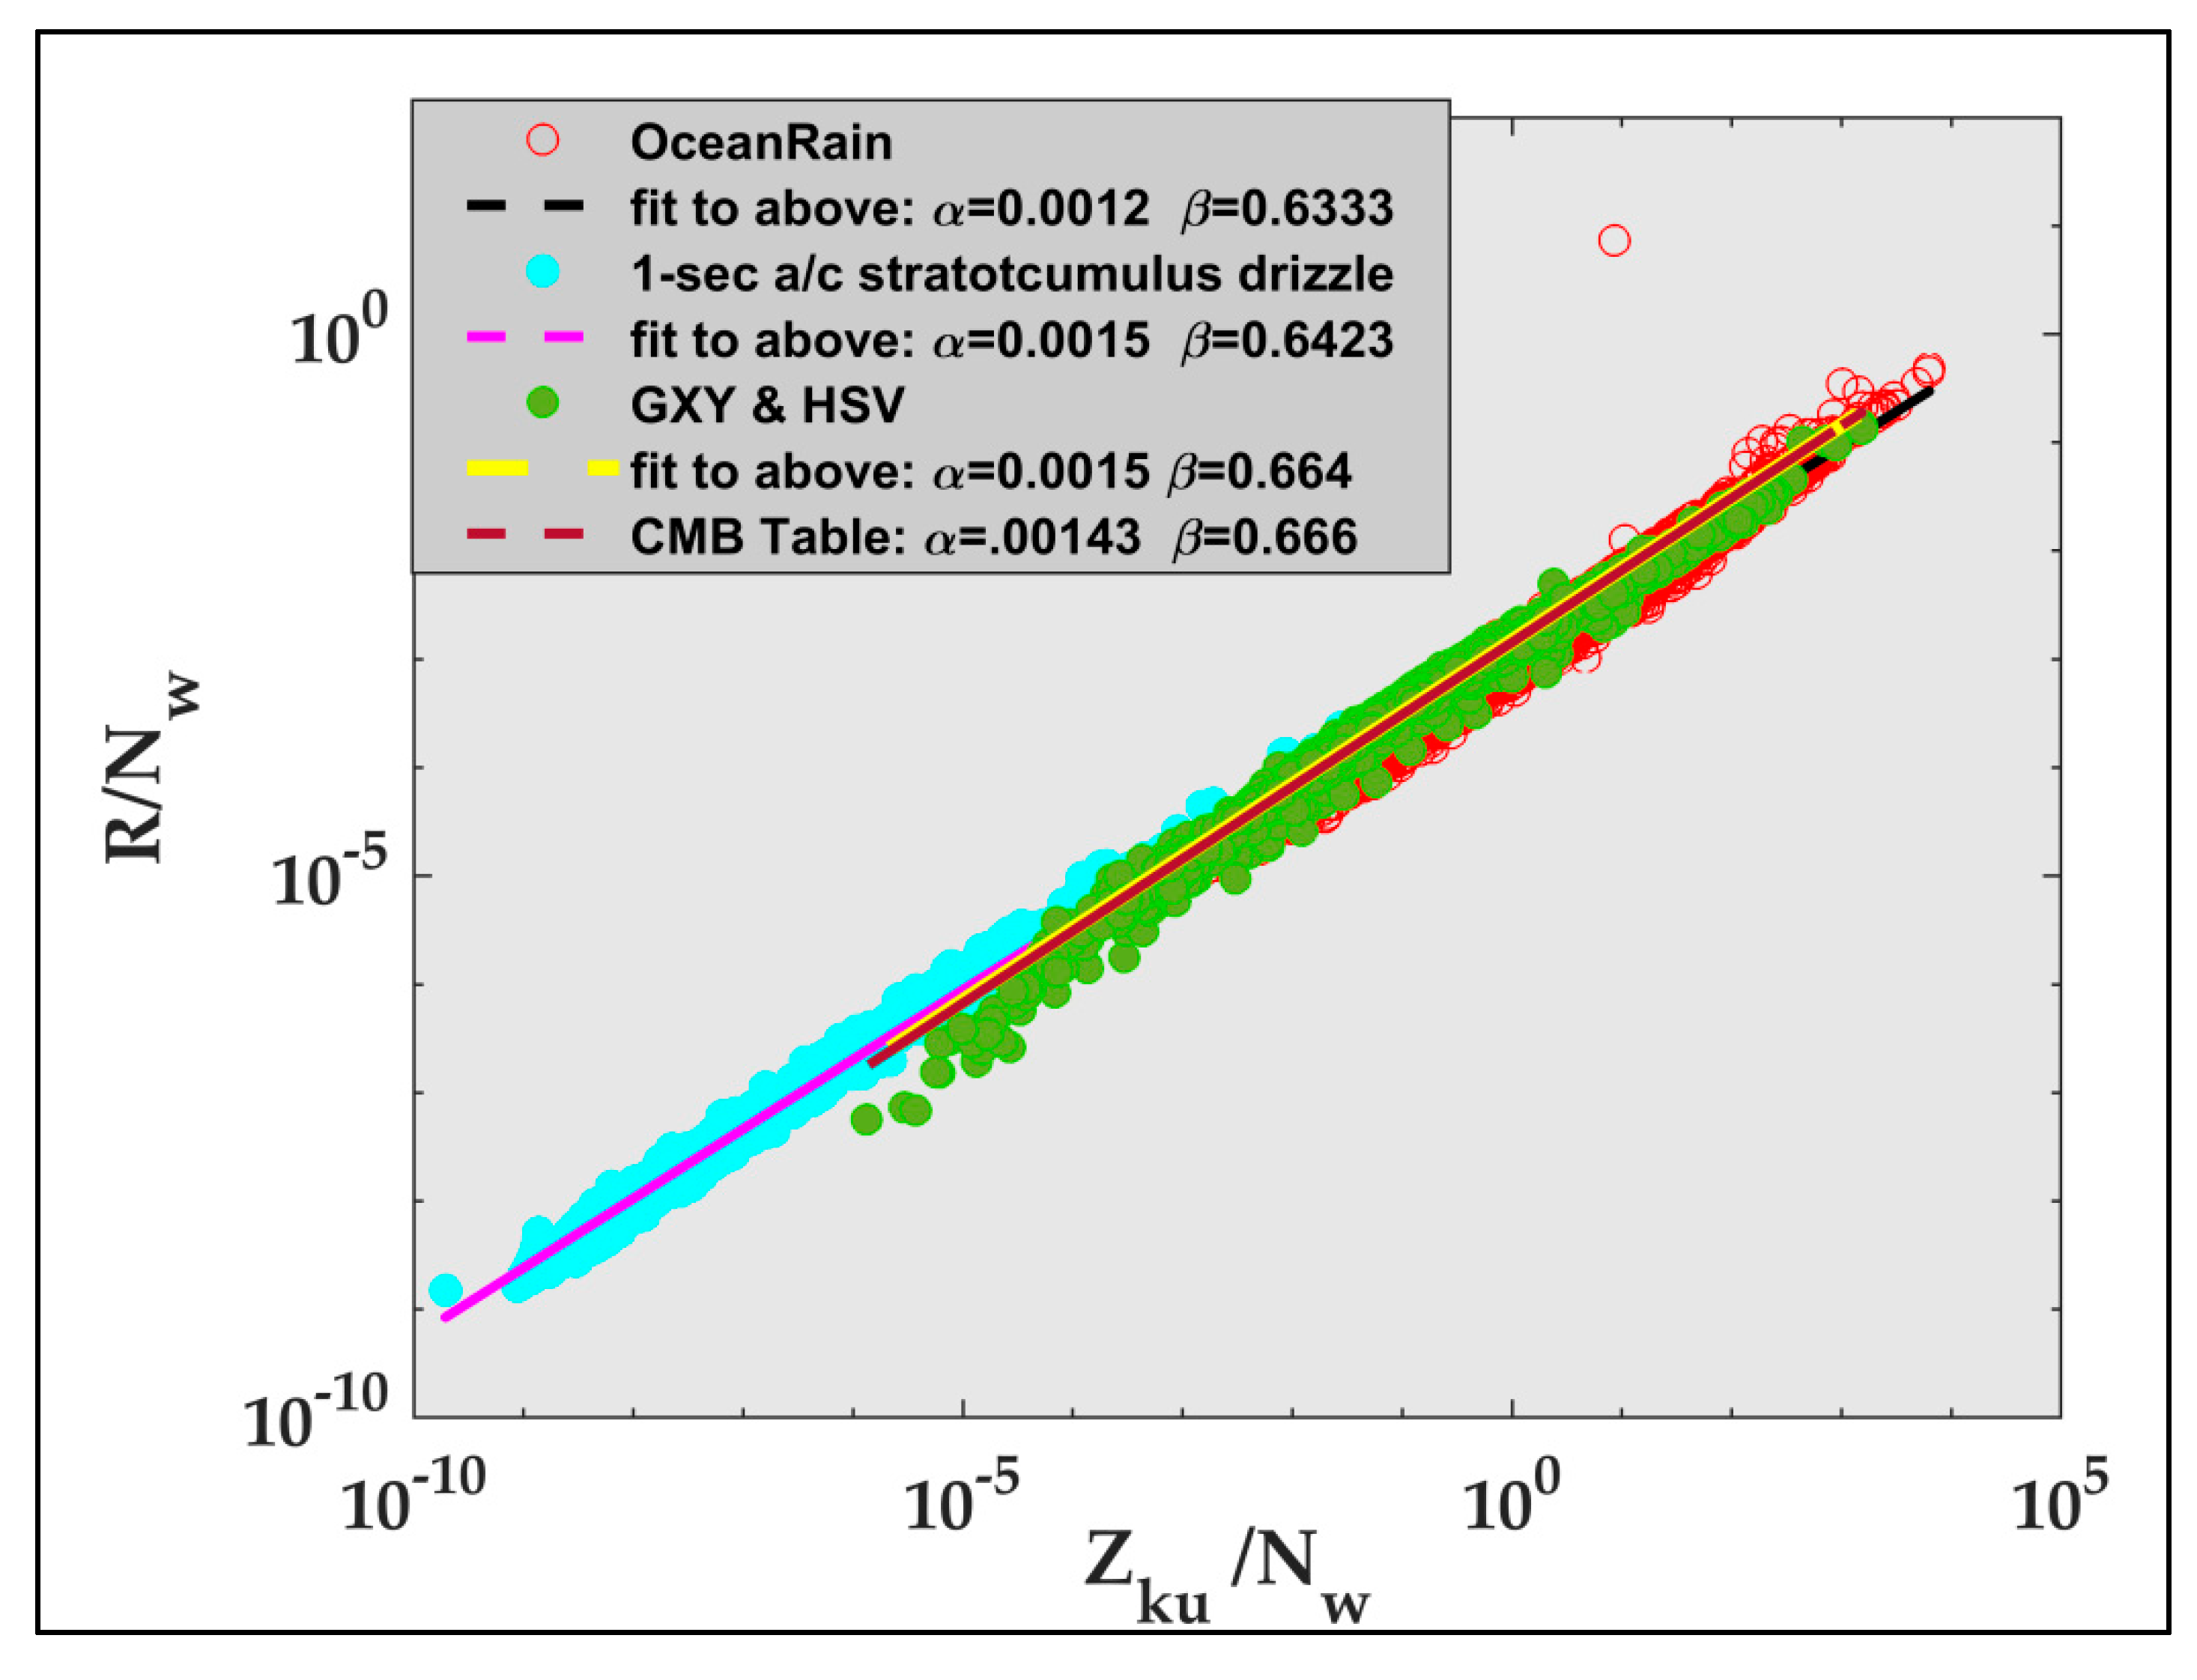
\includegraphics[width=0.9\textwidth]{Figures/fig4.png}
            \end{center}
        \end{figure}
    \end{column}
\end{columns}
\end{frame}
\begin{frame}
\frametitle{The $N_w$ problem. Radar profiling considerations}
\begin{columns}
    \begin{column}{0.55\textwidth}
    \begin{itemize}
        \item Additional constraints can be imposed by using radar
        by considering $N_w$ in the radar profiling context.
        \item That is, the attenuation correction process needs to be
        consistent with the $N_w$ parameter.
        $Z(r)=Z_m(r) /PIA$
        $PIA=(1-\epsilon (N_w) q\int_0^r Z_m^\beta(s)ds)^{1/\beta}$
        \item The analytical PIA needs to be consistent with the
        SRT PIA estimate and Ka-band reflectivity observations 
        when available.
    \end{itemize}
    \end{column}
    \begin{column}{0.5\textwidth}
        \begin{figure}
            \begin{center}
            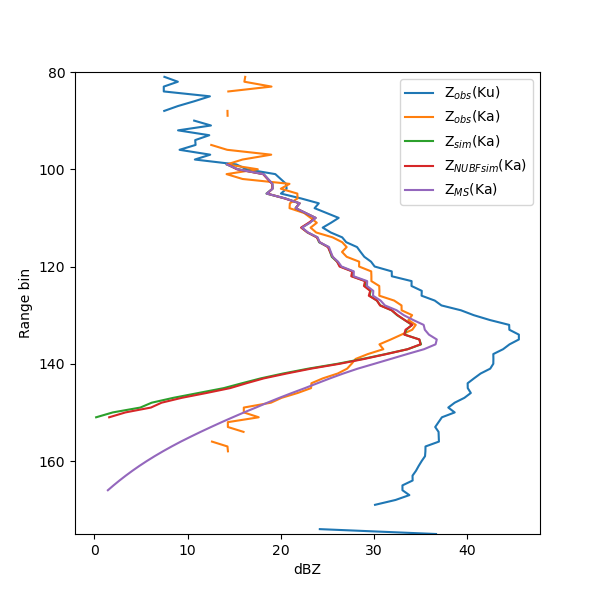
\includegraphics[width=0.9\textwidth]{Figures/fig5.png}
            \end{center}
    \end{figure}
    \end{column}
\end{columns}
\end{frame}
\begin{frame}
\frametitle{The $N_w$ problem. Further considerations}
\begin{itemize}
\item Surface Reference Technique (SRT) PIA is a useful piece of information when reliable.
\item Dual SRT PIA is more reliable than single SRT PIA, except for heavy convection.
\item Over oceans SRT PIA estimates are significantly more reliable than over land.
\item For snow and light rain, SRT PIA estimates are not reliable.
\end{itemize}
\begin{figure}
\begin{center}
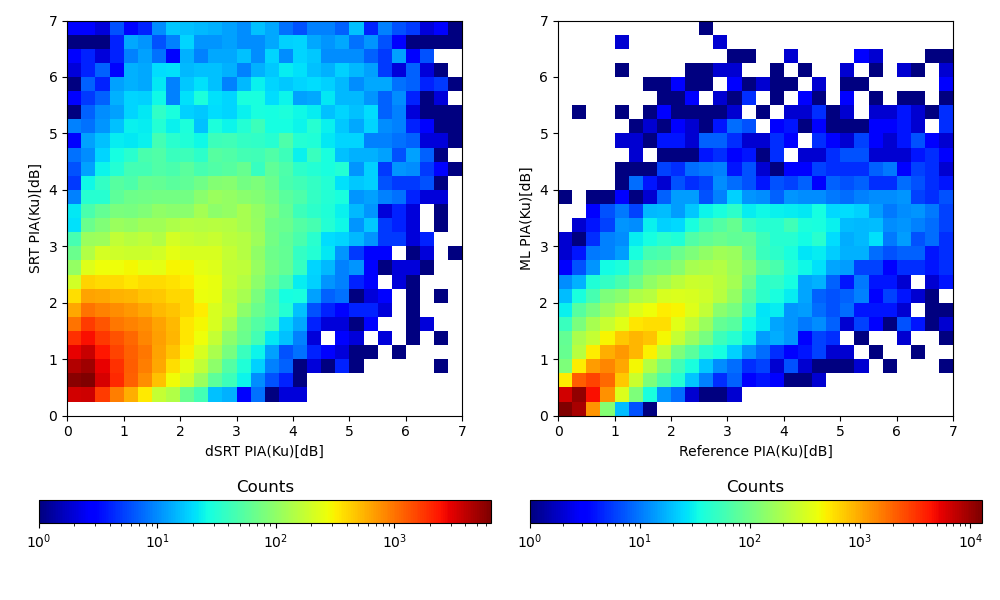
\includegraphics[width=0.85\textwidth]{Figures/fig6.png}
\end{center}
\end{figure}
\end{frame}
\begin{frame}
\frametitle{Snow estimation issues}
\begin{columns}
\begin{column}{0.58\textwidth}
    \begin{itemize}
    \item The variability of $N_w$ is still a problem, but there is very little
    attenuation in snow to use the PIA as a constraint.
    \item When dual frequency observations are available, $D_m$ and hence
    $N_w$ may be estimated from the dual frequency reflectivity ratio (DFR).
    \item However, the DFR may be very noisy.
    \item More robust methods, i.e. Machine-Learning based, may be used 
    to derive to incorporate "in-situ" information and provide
    more accurate estimates.
    \end{itemize}
\end{column}
\begin{column}{0.5\textwidth}
\begin{figure}
\begin{center}
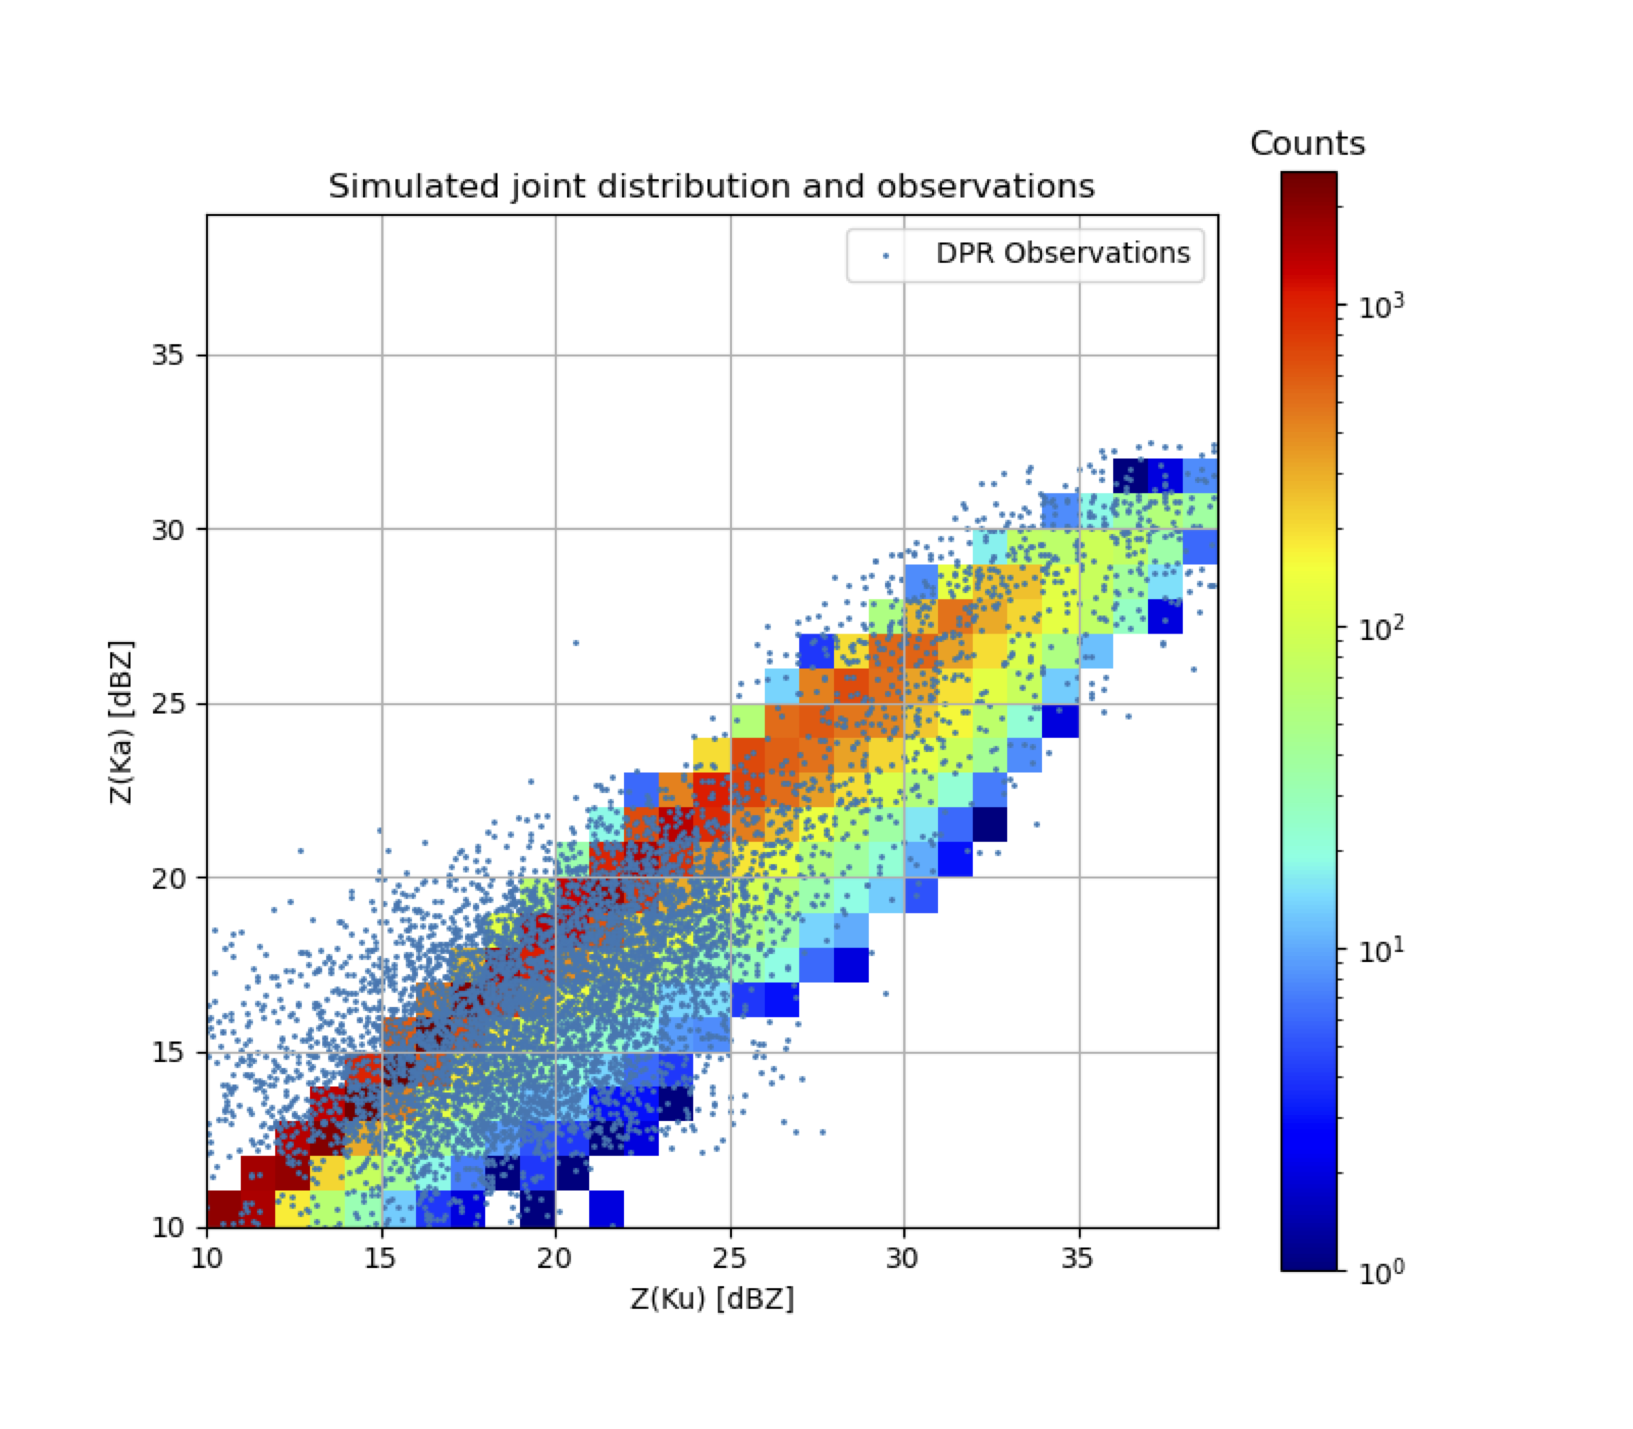
\includegraphics[width=0.9\textwidth]{Figures/fig7.png}
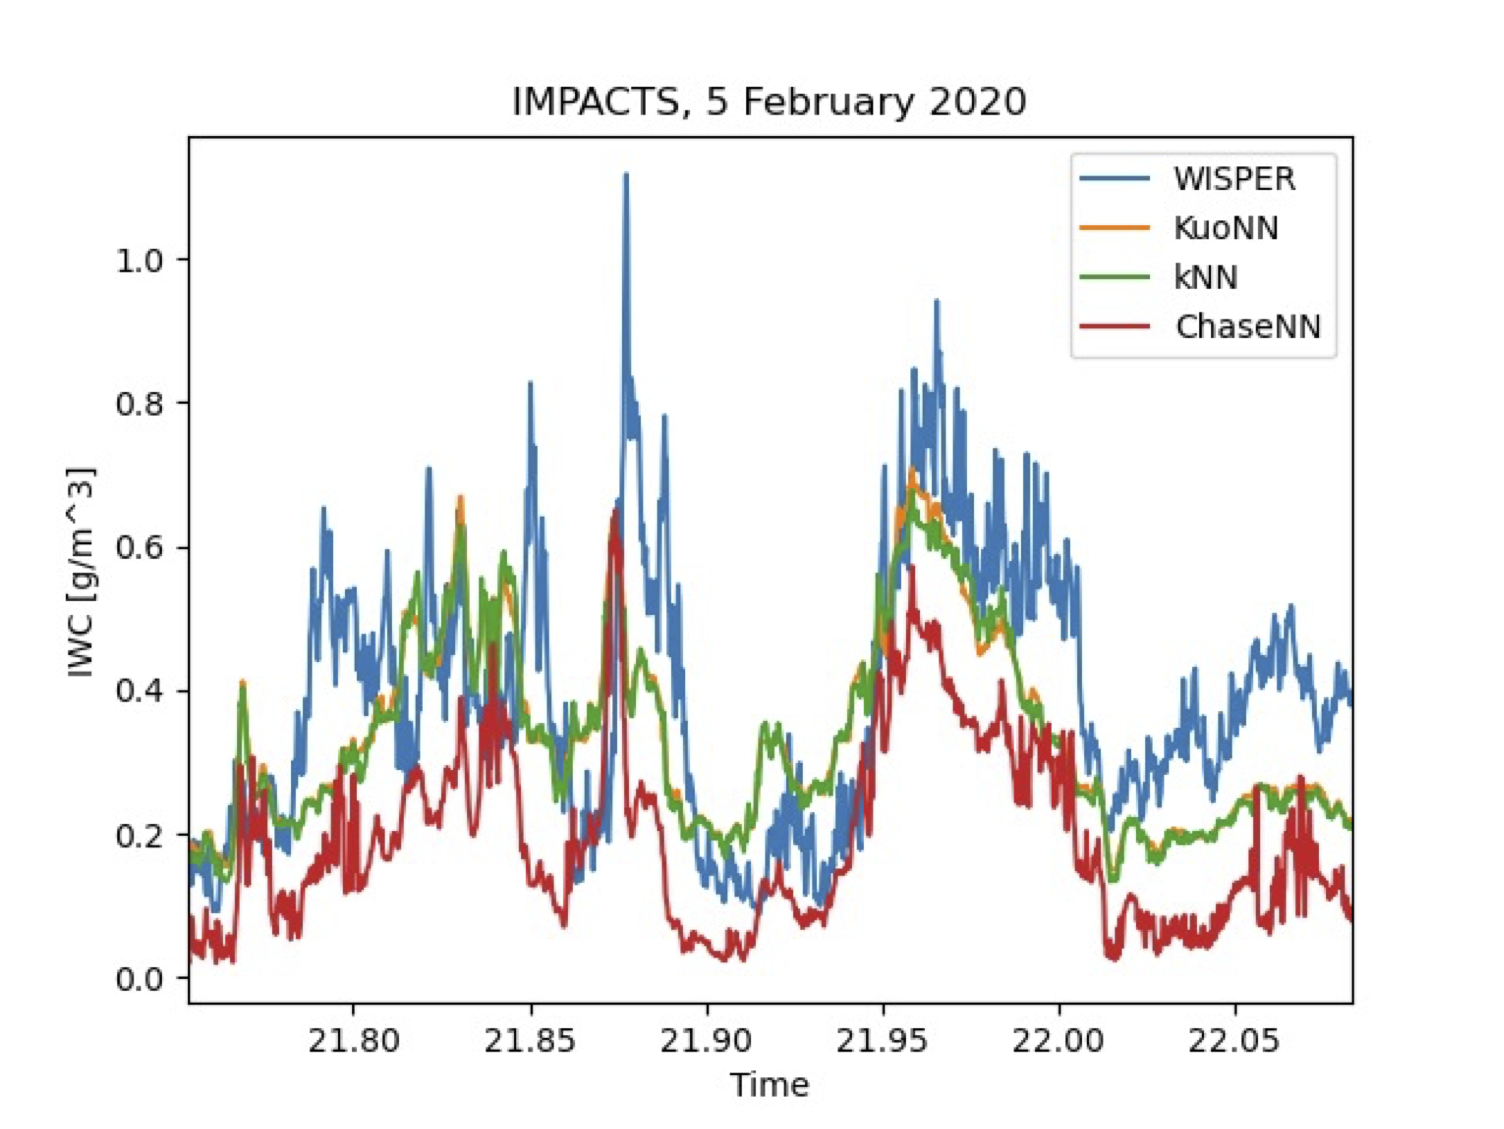
\includegraphics[width=0.9\textwidth]{Figures/Fig8.png}
\end{center}
\end{figure}
\end{column}
\end{columns}
\end{frame}    
\begin{frame}
\frametitle{Ground Clutter}
\begin{columns}
\begin{column}{0.55\textwidth}
    \begin{itemize}
    \item Ground clutter is strong echo in the radar observation caused 
    by the ground.
    \item It can extend up to 2.0 km above the surface and completely 
    obscure the precipitation echo.
    \item Nadir observations are minimally affected 
    and can be used in the development of statistical clutter mitigation 
    methodologies, e.g.
    $pRate(z<z_{cf})=pRate(z_{cf}) \times$
    $pRate_{mean}(z)/pRate_{mean}(z_{cf})$
    \end{itemize}
\end{column}
\begin{column}{0.5\textwidth}
    \begin{figure}
        \begin{center}
        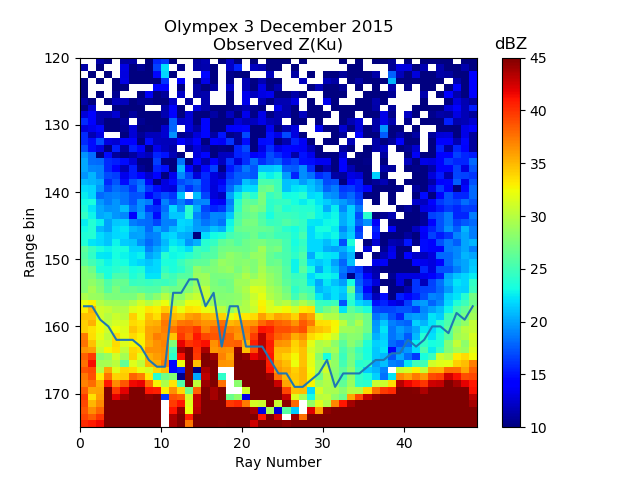
\includegraphics[width=0.9\textwidth]{Figures/fig9.png}
        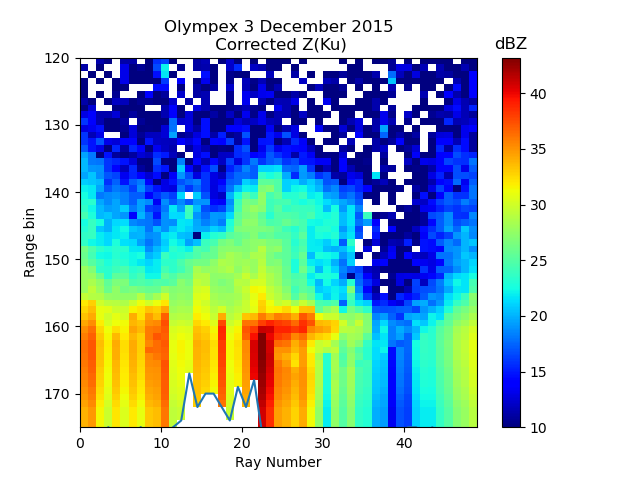
\includegraphics[width=0.9\textwidth]{Figures/fig10.png}
        \end{center}
    \end{figure}
\end{column}
\end{columns}
\end{frame}
\begin{frame}
\frametitle{Impact of Ground Clutter Correction}
\begin{figure}
        \begin{center}
        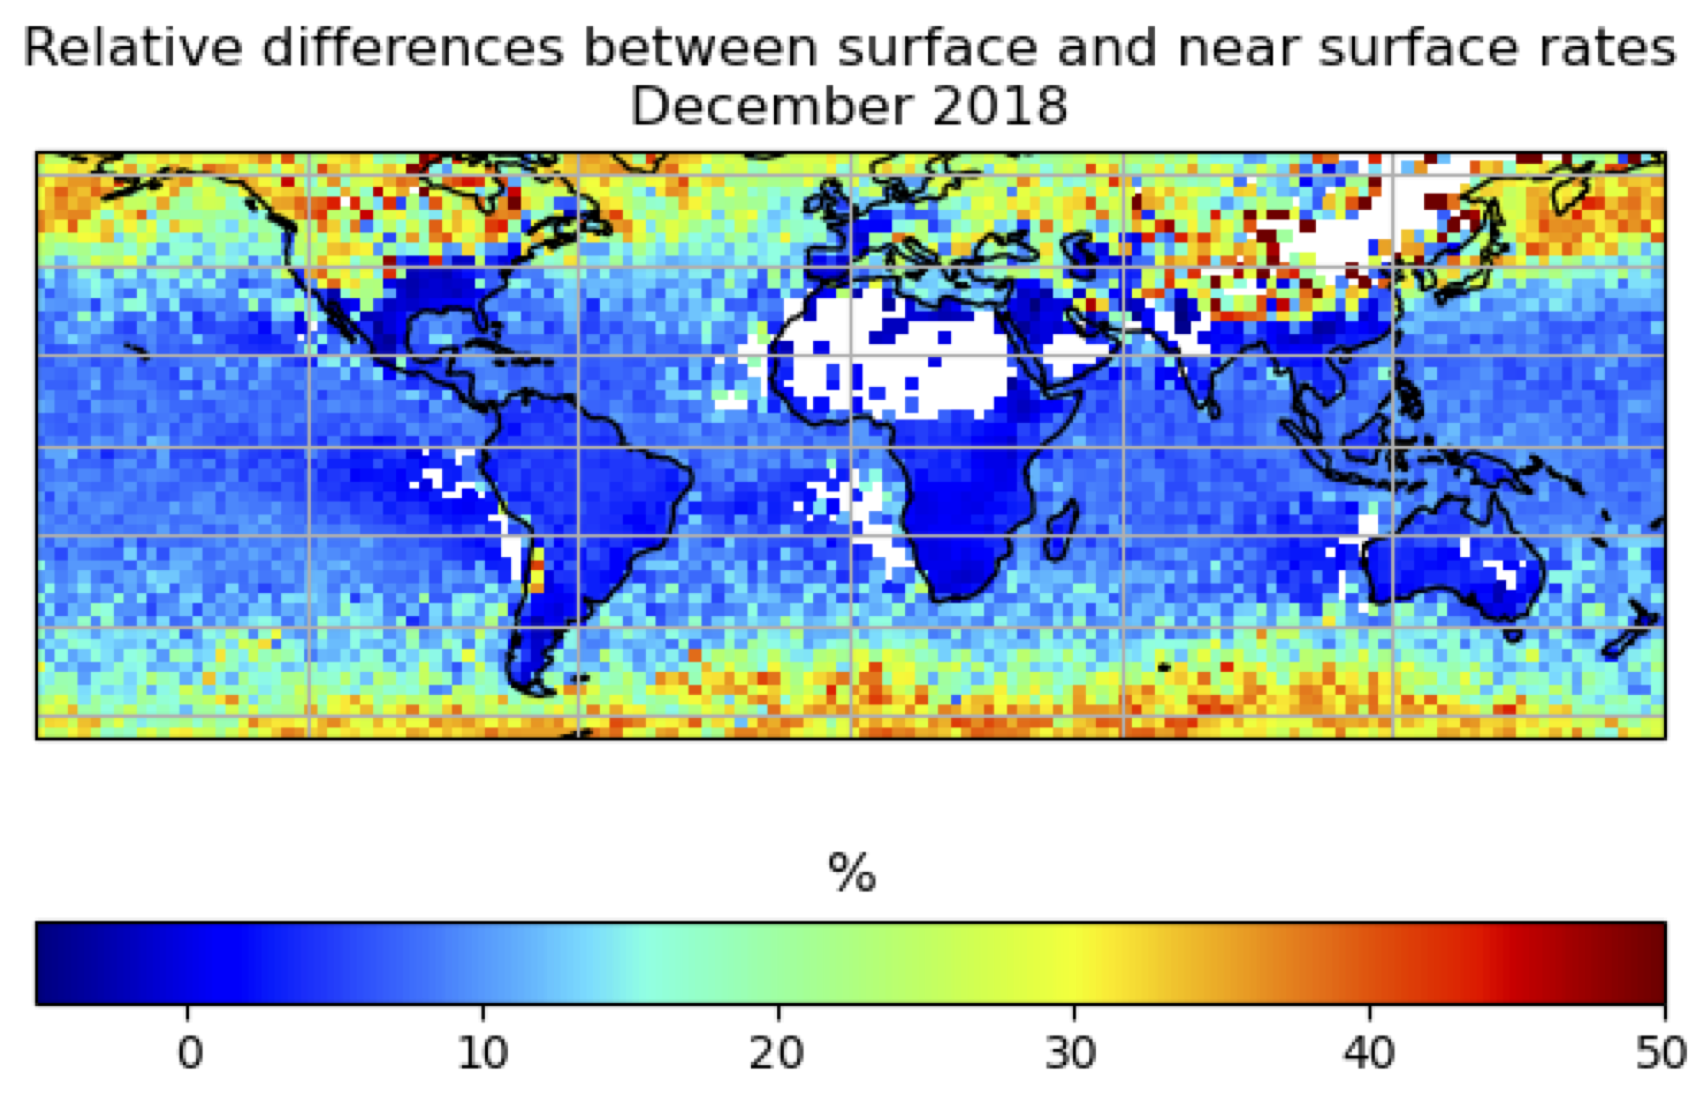
\includegraphics[width=0.9\textwidth]{Figures/fig11.png}
        \end{center}
    \end{figure}
\end{frame}
\begin{frame}
    \frametitle{Light Precipitation}
    \begin{columns}
        \begin{column}{0.55\textwidth}
            \begin{itemize}
            \item The DPR does not miss all the light precipitation associated with a given point in the Tb-space
            \item An empirical algorithm may be derived from collocated Tbs and DPR retrievals
            \item The empirical algorithm is to be applied only when the DPR does not detect precipitation. When estimates are greater than 0, a decision is required.
                
            \end{itemize}
        \end{column}
        \begin{column}{0.5\textwidth}
            \begin{figure}
                \begin{center}
                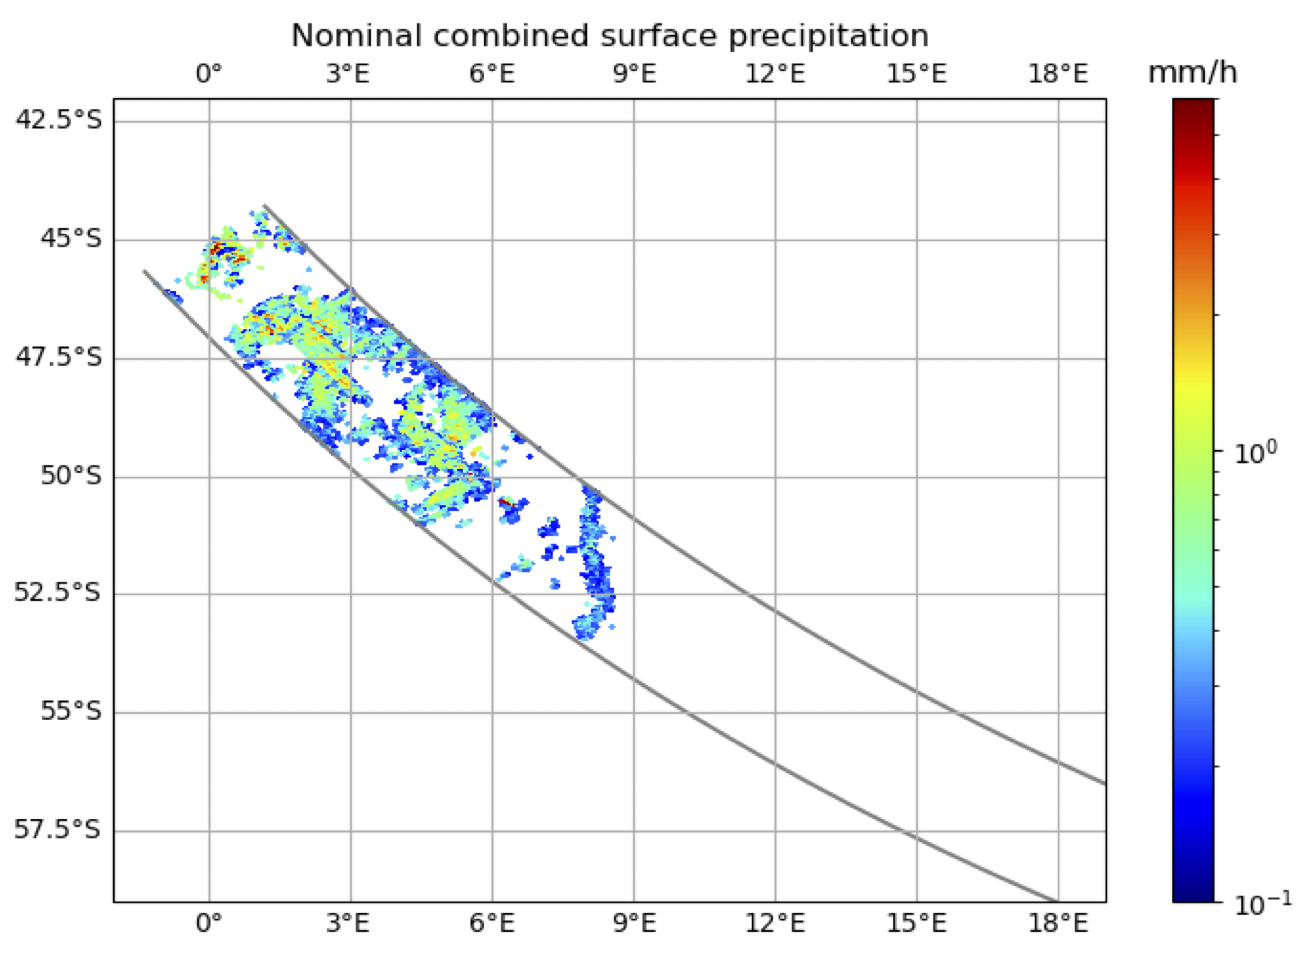
\includegraphics[width=0.9\textwidth]{Figures/fig12.png}
                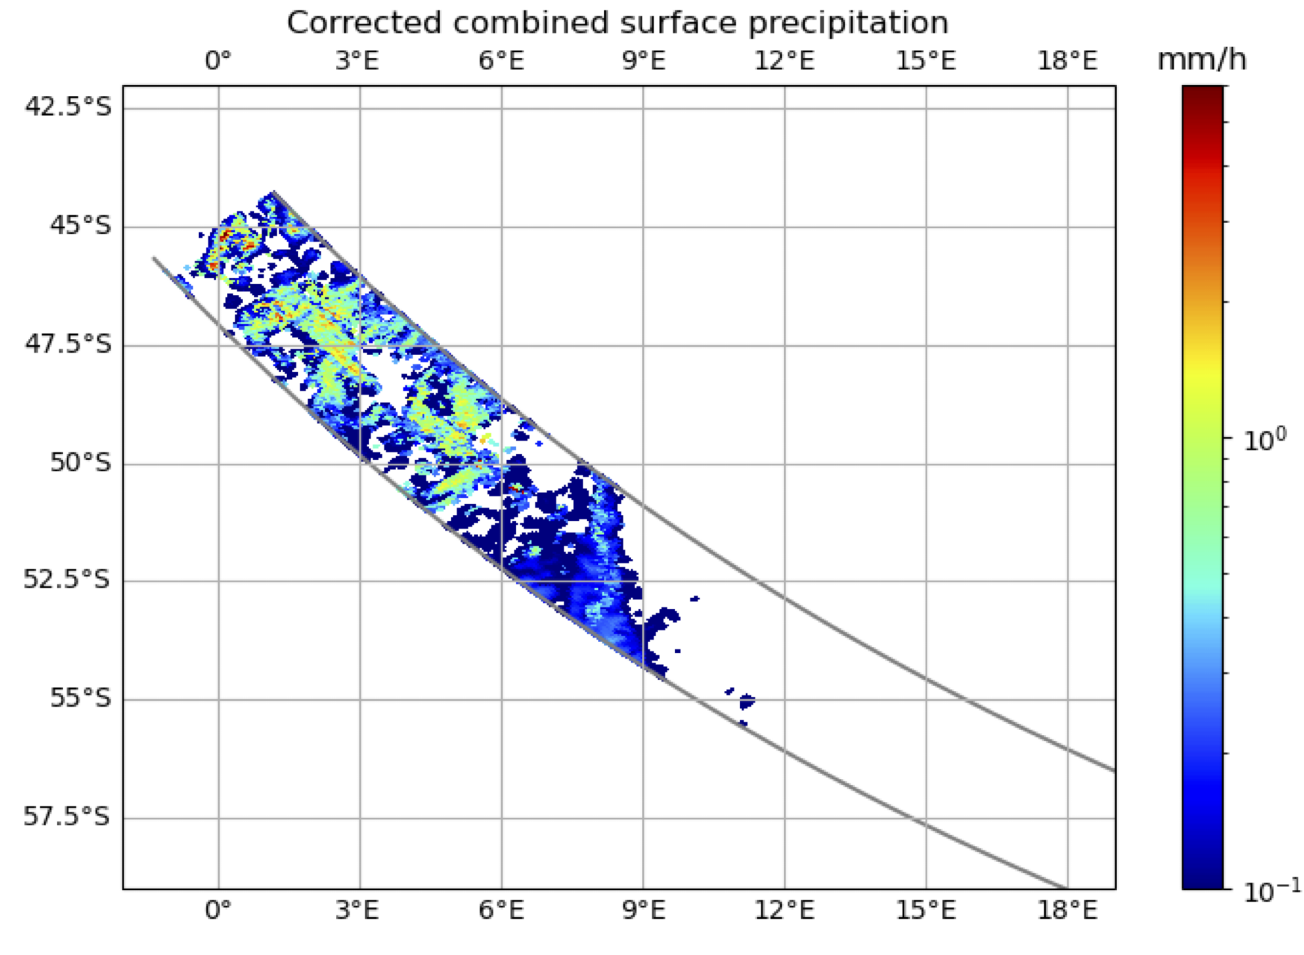
\includegraphics[width=0.9\textwidth]{Figures/fig13.png}
                \end{center}
            \end{figure}
        \end{column}
    \end{columns}
\end{frame} 
\begin{frame}
    \frametitle{Summary and Conclusions}
    \begin{itemize}
        \item Although the most accurate at the instantaneous level, space-borne radar precipitation 
        estimates affected by multiple types of uncertainties.
        \item Even when dual frequency observations are available, the 
        estimation problem is still posed.
        \item Parameterizations and "a priori" information derived 
        from ground observations may be used to mitigate the uncertainties.
        \item However, the process is not trivial and requires a sustained
        long-term effort.
    \end{itemize}
\end{frame}
\end{document}
